\documentclass[12pt, a4paper]{article}

% Font & text
\usepackage{times}
\usepackage[utf8]{inputenc} 
\setlength{\parindent}{0in}
\usepackage{hyperref}
\hypersetup{%
    pdfborder = {0 0 0}
}
\usepackage{caption}
\usepackage{subcaption}
\usepackage{float}

% Math
\usepackage{amsmath}
\usepackage{amssymb}
\usepackage{mathtools}

\newcommand{\im}{\mathrm{Im}}
\newcommand{\p}[1]{\left( #1 \right)}
\newcommand{\lr}[3]{\left#1 #3 \right#2}
\newcommand{\st}{\mathrm{s.t.}}
\newcommand{\N}{\mathbb{N}}
\newcommand{\Z}{\mathbb{Z}}
\newcommand{\B}{\mathbb{B}}
\newcommand{\R}{\mathbb{R}}
\newcommand{\atan}{\mathrm{atan}}
\newcommand{\atantwo}{\mathrm{atan2}}
\newcommand{\Oh}{\mathcal{O}}
\newcommand{\lineseg}[1]{\overline{#1}}

% Source code
\usepackage{listings}
\usepackage{color}

\newcommand{\addcode}[1]{
\subsection*{#1}
\lstinputlisting[language=python, xleftmargin=-5em,xrightmargin=-5em]{../#1}
}

\lstset{
    language=Python,
    showstringspaces=false,
    breaklines=true,
    breakatwhitespace=false,
    formfeed=\newpage,
    tabsize=4,
    numbers=left,
    numbersep=5pt,
    numberstyle=\tiny\color{gray},
    commentstyle=\itshape\color{gray},
    keywordstyle=\bfseries\color{blue!40!black},
    identifierstyle=\color{black},
    stringstyle=\color{green!50!black},
    basicstyle=\ttfamily,
    morekeywords={lambda}
}


% Algorithms
\usepackage[noend]{algpseudocode}
\usepackage{algorithm}

\makeatletter
\def\BState{\State\hskip-\ALG@thistlm}
\makeatother


% Proofs
\usepackage{amsthm}

\newtheorem{theorem}{Theorem}[section]
\newtheorem{corollary}{Corollary}[theorem]
\newtheorem{lemma}[theorem]{Lemma}

\renewcommand\qedsymbol{$\blacksquare$}


% Page, Header & Footer
%\usepackage{geometry}
\pagestyle{empty}
\usepackage{lastpage}
\usepackage{fancyhdr}
\pagestyle{fancy}
\fancyhead{}
\fancyhf{}
\renewcommand{\headrulewidth}{0pt}
\cfoot{}
\rfoot{\thepage\ of \pageref{LastPage}}
\rhead{}

% Images
\usepackage{tikz}

\usepackage{titling}
\date{26th October 2016}
\author{Jon Kingo Christensen}
\def\identification{Jon Kingo Christensen, 180491, jonch10@student.sdu.dk}
\def\courseCode{DM803}
\def\courseTitle{Advanced Datastructures}
\def\lectorLabel{Teacher:}
\def\lector{Kim Skak Larsen}
\def\universityName{Syddansk Universitet}
\def\papertitle{Assignment 1}
\def\papersubtitle{\courseTitle}
\title{\papertitle{} - \papersubtitle{}}




% ============ %
\begin{document}
%\maketitle

\begin{tabular}{@{}l}
\universityName{} \\
\lectorLabel{} \lector{}
\end{tabular}
\hfill
\begin{tabular}{r@{}}
\courseTitle{} (\courseCode{}) \\
\thedate{}
\end{tabular}

\bigskip

% Frontpage Title
\begin{center}
    \Huge{\papertitle{}} \\
    \Large{\papersubtitle{}}
\end{center}
\normalsize{}

\begin{center}
    \identification{}
\end{center}

%\bigskip

%\newpage

%\restoregeometry{}



\section*{Specification}
This report describes the implementation of scapegoat trees and skip lists in the programming language python. The report mostly 
discusses test results from comparing the two datastructures looking only at number of comparisons of keys. 
And not the actual run times in real time.


\section*{Implementation details}
The datastructures have been implemented in python version 3.4.3 and this is the version that should be run for testing it.
On the IMADA terminal machines this is done using python3.

\medskip

The programs read from \texttt{stdin} and writes to \texttt{stdout}, an example of running the scapegoat Tree using an input file and writing
to an output file can be seen below:
\begin{lstlisting}[language=bash]
  python3 scapegoatTree.py < inputfile > outputfile
\end{lstlisting}

\medskip

The comparisons are counted by, for each query, incrementing when searching through a datastructure and 
a comparison between two keys are made. In skiplist it was doubtful whether to include the comparison with the "tail" element. 
But that comparison is also counted.

\medskip

In the implementation of skip lists. Instead of initialising an empty array of size equal to the level of a node, 
for pointers, dynamic lists are used. 
This is not a big change from the article on skip lists as the time complexity of push and pop is amortized $\mathcal{O}(1)$.

\medskip

The restructuring of subtrees in scapegoat trees have been done differently from the article on scapegoat trees. 
Instead of using a linked list, the tree is first flattened by a recursive flatten on left child, then the node itself, then a recursive flatten
on the right child. The tree is then reconstructed by taking the element in the middle of the list, recursively creating its left subtree from the list
of nodes to the left of the middle, and its right subtree from the list of node to the right of the subtree.

\medskip

42 has been used as the random seed for tests in this report.
The default value of $\alpha$ in the scapegoat tree is 0.75, and the default value of p in the skip list is 0.25

\section*{Testing}
The program maketest.py has been written to generate examples for the tests given in this section. 
Specifically \texttt{test1} was used for the average search complexity.
To evaluate p values in skip lists, and variations in search complexity \texttt{test2} was used. 
And finally test3 and others were used to look at size and frequency of rebuilds in scapegoat trees.
The \texttt{manual.txt} document describes how to use this tool if the tests needs to be recreated.

\subsection*{Average search complexity}
The average search times have been investigated by repeatingly inserting 50 elements into the data structure, and then searching 50 times for some 
element in the datastructure (including previously added elements). Then taking the average of the comparisons used for each of the 50 searches.
Fig. \ref{avgsearch} shows the results of doing this up until 100.000 elements have been inserted.

\begin{figure}[H]
    \centering
    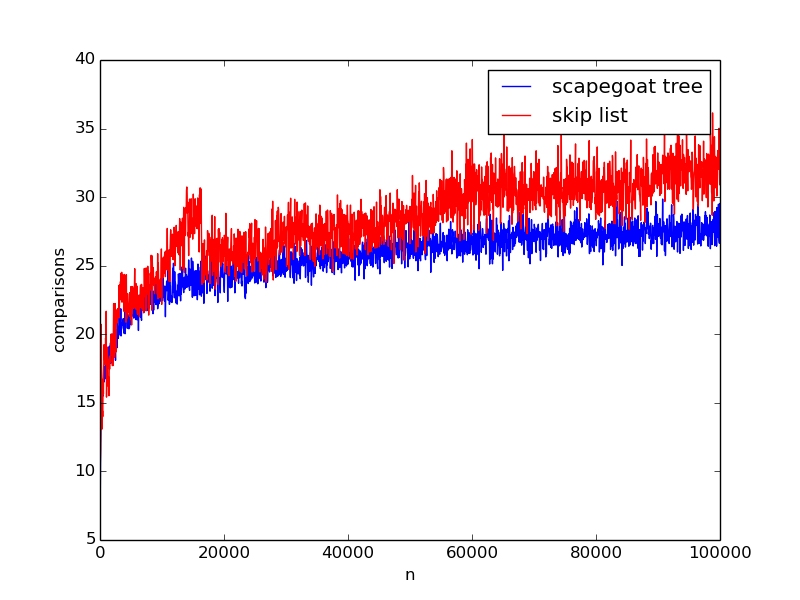
\includegraphics[width=1\textwidth]{averagesearch.png}
    \caption{scapegoat tree and skip list average search times.}
    \label{avgsearch}
\end{figure}

To try and demonstrate that the algorithm is logarithmic. The y-axis of the graph has been scaled logarithmically in Fig. \ref{logscale}

\begin{figure}[H]
    \centering
    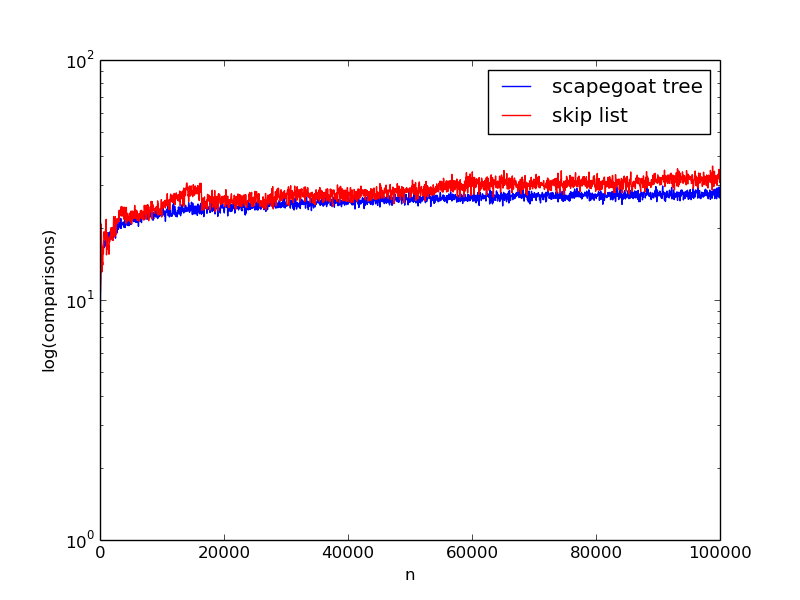
\includegraphics[width=1\textwidth]{logscale.png}
    \caption{scapegoat trees and skip lists logarithmically scaled.}
    \label{logscale}
\end{figure}

The linear growth on a logarithmic scale could suggest that the search time in fact does grow logarithmically. To find an approximation 
of the constant in front of the log, one could divide all the comparison results with the logarithm of the size of the datastructure at the time
of the searches. This could reveal some constant, due to the fact that $\frac{k\cdot log(n)}{log(n)}=k$. These calculations have been done and the results
can be seen in Fig. \ref{divilog}

\begin{figure}[H]
    \centering
    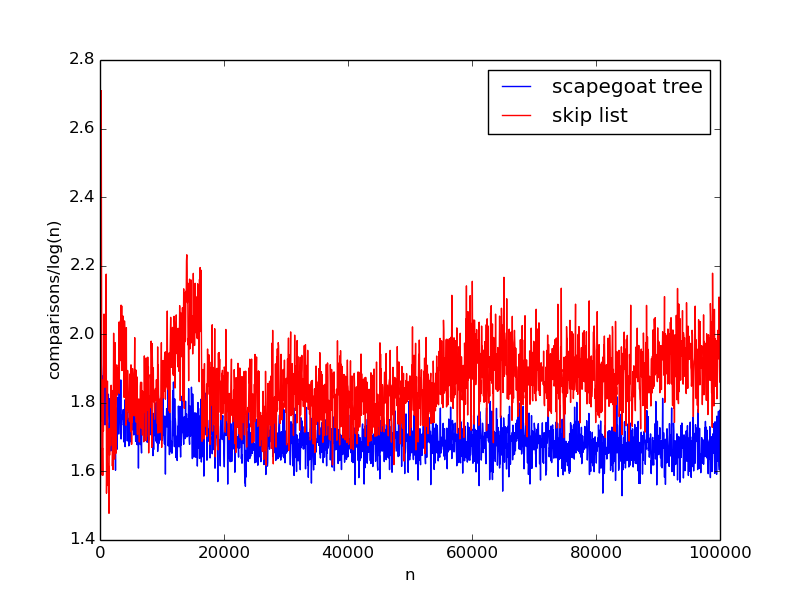
\includegraphics[width=1\textwidth]{dividedlog.png}
    \caption{scapegoat trees and skip lists, where results are divided by the logarithm of the input size.}
    \label{divilog}
\end{figure}

This graph would suggest that the constant for the scapegoat trees lie somewhere between 1,6 and 1,8. and the skip lists constant between 1,8 and 2,1.

\medskip

To evaluate the p used in the skip list, one can try to look at what the constant is in front of the logarithm for each p. 
This was done with 100.000 insertions followed by 100.000 searches, the average of the searches was then found and divided by the logarithm of 
the input size. The results of these can be seen in Table \ref{table}.
\begin{table}
\centering
\caption{table of p's and their constants}
\label{table}
\begin{tabular}{|c|c|c|}
\hline
p                & Constant \\
\hline
1/2 & 1.9039   \\
\hline
1/e  & 1.7540   \\
\hline
1/4  & 1.9380   \\
\hline
1/8  & 2.8625   \\
\hline
1/16 & 3.5809  
\hline
\end{tabular}
\end{table}

The constants follow the same trend as in the article, where it first goes down, then starts growing again. although here it appears that the 
p value of a half is a bit better than that of a quater, unlike the article. The values are also generally larger than in the article.


\subsection*{Variation in search complexity}
The variation of the search complexity can be found by doing many searches and recording for each i, how many searches required i comparisons.
This has been evaluated by creating a random shuffle of 100.000 integers and inserting them. Then all the same integers are searched for.
This eliminates duplicate searches which is not as relevant here as getting the full spectrum of search complexities is. The results 
can be seen in Fig. \ref{variation}

\begin{figure}[H]
    \centering
    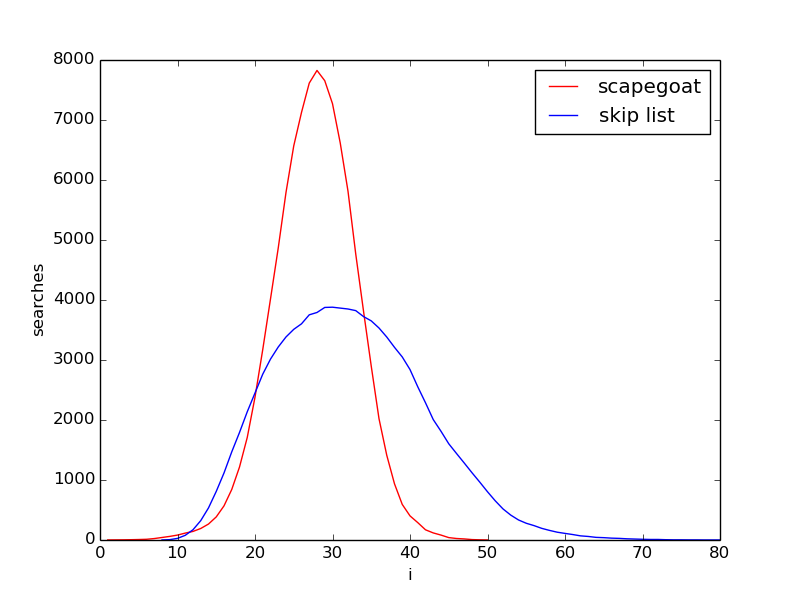
\includegraphics[width=1\textwidth]{variation.png}
    \caption{variation of search complexities for scapegoat trees and skip lists.}
    \label{variation}
\end{figure}

The graph shows that scapegoat trees has a more narrow variation, and it's generally a bit lower than skip lists.

\subsection*{Scapegoat tree restructurings}
Testing with counting restructurings of subtrees, showed that the amount of restructurings varied highly dependant on the input. 
Sorted order input gives many even sized restructurings, while uniformly random inputs give very few restructurings, where some could get very big.
but most were still quite small. This have not been graphed due to the extreme outliers giving an incromprehensible graph. 



\section*{Conclusion}
Overall the datastructures are both quite fast, comparison wise the scapegoat tree wins on the tests performed in the report. But in overall time 
of the program, the skip lists were quite faster than the scapegoat trees when having very large inputs.

























\end{document}
